\section{Ejercicio 4}
En este apartado se realizar\'a el dise\~no de un circuito adaptador de se\~nal, por ejemplo para que esta pueda ser le\'ida por un microcontrolador. Para tal fin es necesario conocer tanto los par\'ametros de entrada como los de salida, as\'i como las limitaciones presentes en el dise\~no.

\subsection{Se\~nal de entrada}
La se\~nal de entrada del circuito provendr\'a de un \textsc{mpx2010dp}. Este es un sensor de presi\'on que opera de forma piezorresistiva. Esto significa que la magnitud ser\'a medida indirectamente a trav\'es de un cambio en la resistencia de un resistor calibrado. Dicha diferencia est\'a dada por una peque\~na deformaci\'on en la geometr\'ia del resistor debido a la presi\'on ejercida por un flu\'ido hidr\'aulico encapsulado en el interior del sensor propiamente dicho.

\begin{figure}[H]
    \centering
    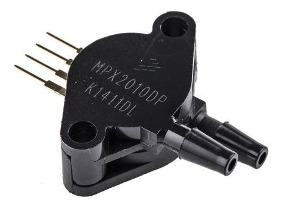
\includegraphics[width=0.5\textwidth]{../EJ4/resources/mpx2010dp.png}
    \caption{Sensor \textsc{mpx2010dp}}
    \label{fig:EJ4_mpx2010dp_image}
\end{figure}

Como se puede observar en la imagen anterior el sensor posee dos entradas de fluido. Esto es as\'i dado que el mismo mide la presi\'on de una de las entradas, en relacion a la otra. Esto es precisamente \'util para medir la presi\'on manom\'etrica de un determinado fluido (esto es, su presi\'on en relaci\'on a la atm\'osfera. De esta forma, el sensor entrega una se\~nal de tensi\'on que ser\'a lineal y proporcional a esta diferencia de presi\'on. Esto se puede observar en la figura~\ref{fig:EJ4_mpx2010dp}.

\begin{figure}[H]
    \centering
    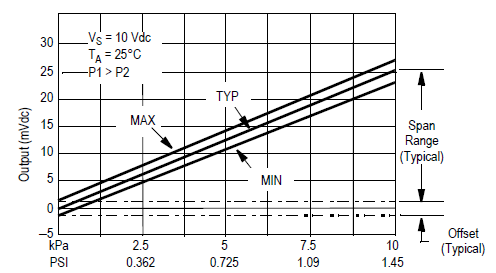
\includegraphics[width=0.5\textwidth]{../EJ4/resources/mpx2010dp_out.png}
    \caption{Salida del \textsc{mpx2010dp} en funci\'on a la diferencia de presi\'on}
    \label{fig:EJ4_mpx2010dp_out}
\end{figure}

Como se puede apreciar en la figura anterior, la salida del sensor oscila entre $0V$ y $25mV$ aproximadamente. Este rango de tensi\'on se ubica en el orden de magnitud del piso de ruido, por lo que emplear este sensor sin amplificar resultar\'ia en mediciones err\'oneas y probablemente aleatorias (en funci\'on del tipo de ruido presente en el lugar de operaci\'on del sensor). A\'un asi realizando una amplificaci\'on de la salida hay que tener en cuenta que el circuito que se encargue de ello debe ser lo suficientemente inmune al ruido como para que la salida del mismo sea representativa de la presi\'on ejercida sobre el sensor.


Por esta raz\'on es apropiado emplear un circuito que contenga un amplificador de instrumentaci\'on, de forma tal de minimizar el error de medida a la salida. 

\subsection{Amplificador de instrumentaci\'on}

Un amplificador de instrumentaci\'on es un circuito compuesto por amplificadores operacionales y resistores que satisface los siguientes requerimientos:

\begin{enumerate}
		\item Impedancias de entrada en modo com\'un y diferencial altas (idealmente infinitas).
		\item Impedancias de salida muy bajas (idealmente nulas).
		\item Ganancia alta y relativamente estable.
		\item Alto grado de CMRR \textit{(Common Mode Rejection Ratio)}
\end{enumerate}

Estas caracter\'isticas hacen al amplificador especialmente apto para aplicaciones cuyas se\~nales sean d\'ebiles, como por ejemplo en el campo de la medicina. Tambi\'en es ideal para amlpificar el sensor \textsc{mpx2010dp}. En l\'ineas generales existen dos circuitos de instrumentaci\'on: uno que utiliza dos amplificadores operacionales y otro que usa tres.

\begin{figure}[H]
    \centering
    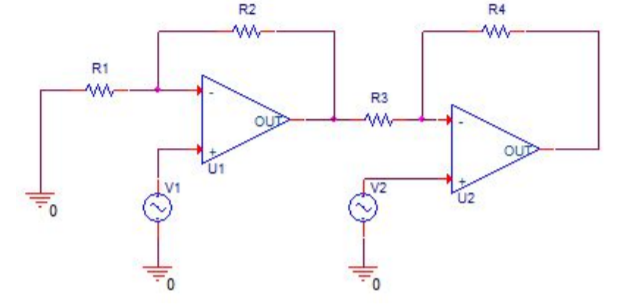
\includegraphics[width=0.9\textwidth]{../EJ4/resources/instrumental_2opamp.png}
    \caption{Amplificador de instrumentaci\'on de 2 op-amp}
    \label{fig:EJ4_instrumental_2opamp}
\end{figure}

\begin{figure}[H]
    \centering
    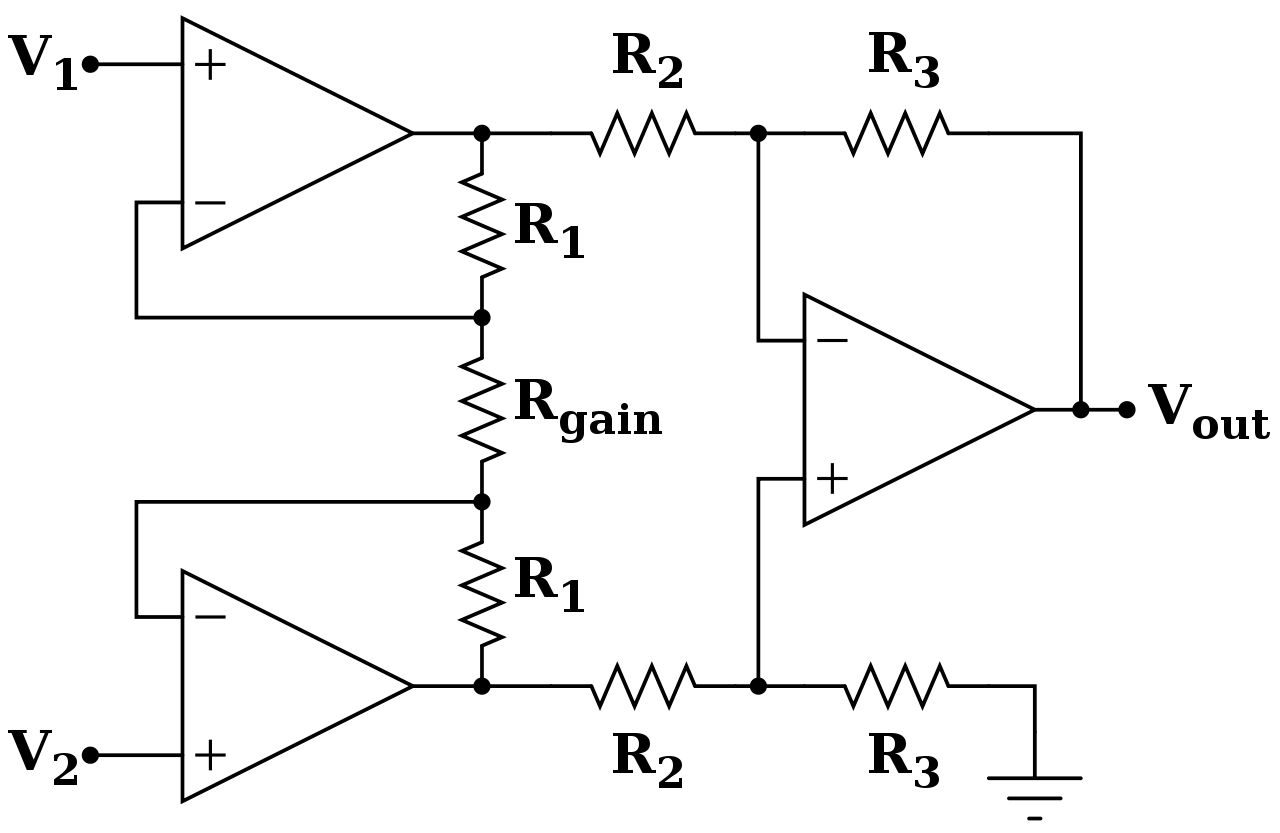
\includegraphics[width=0.9\textwidth]{../EJ4/resources/instrumental_3opamp.png}
    \caption{Amplificador de instrumentaci\'on de 3 op-amp}
    \label{fig:EJ4_instrumental_3opamp}
\end{figure}
 
 La principal ventaja de la configuraci\'on dual es que obviamente se requieren menos amplificadores operacionales. Por otro lado, comparado con la configuraci\'on de tres op-amp el circuito tratar\'a a las dos entradas ($V_1$ y $V_2$) de forma asim\'etrica, debido al tiempo de propagaci\'on existente entre las dos etapas. Este factor hace que el coeficiente de CMRR se degrade en rango de frecuencias elevado. Esta variable no afecta al diseño, dado que se trabaja con tensi\'on en corriente continua y constante. Explicado esto, se utilizar\'a la configuraci\'on de op-amp dual.
 
 
Para este circuito se realiza un an\'alisis de forma tal de conseguir la ganancia del sistema. Para ello se modelizan las entradas en modo diferencial como dos fuentes de valor $\frac{v_d}{2}$ y una tensi\'on $V_{cm}$ que simboliza una componente presente en ambas entradas de igual forma, que por ejemplo puede ser la representaci\'on de ruido en las se\~nales. El modelo se presenta a continuaci\'on.

\begin{figure}[H]
    \centering
    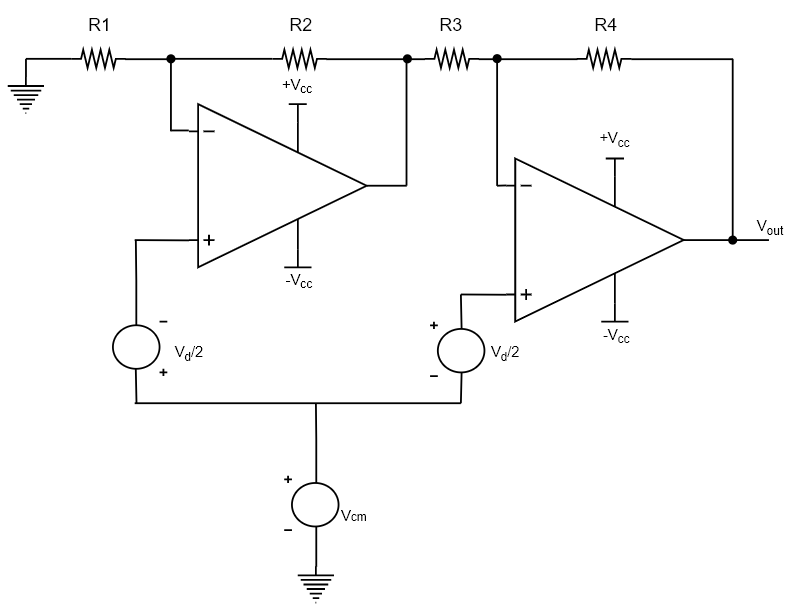
\includegraphics[width=0.9\textwidth]{../EJ4/resources/2opamp_difmode_gain.png}
    \caption{C\'alculo de ganancia en modo diferencial}
    \label{fig:EJ4_2opamp_difmode_gain}
\end{figure}

Si se aplica el principio de superposici\'on sobre las dos entradas no inversoras de los amplificadores operacionales se obtiene la siguiente ecuaci\'on, que refleja la ganancia en modo diferencial del sistema, en funci\'on de los resistores que lo componen.

\begin{equation}
V_{out} = \frac{v_d}{2} \cdot \left( 1 + \frac{2R_4}{R_3} + \frac{R_2 \cdot R_4}{R_1 \cdot R_3} \right) + v_{cm} \cdot \left( 1 - \frac{R_2 \cdot R_4}{R_1 \cdot R_3} \right)
\label{EJ4_vout}
\end{equation}

En la ecuaci\'on anterior se pueden distinguir dos t\'erminos: por un lado, uno dependiente de $v_d$ (que es la se\~nal que se busca amplificar), y por otro uno dependiente de $v_{cm}$ cuyo impacto se busca minimizar. Para lograr esto \'ultimo, se puede asumir una condici\'on de puente entre los resistores,  lo que deriva en la siguiente equivalencia.

\begin{equation}
\frac{R_1}{R_2} = \frac{R_4}{R_3} 
\label{EJ4_condicion_puente}
\end{equation}

De esta forma, se simplifica la expresi\'on de la ecuaci\'on~\ref{EJ4_vout} y se obtiene

\begin{equation}
v_{out} = v_d \cdot \left( 1+\frac{R_1}{R_2} \right) = v_d \cdot \left( 1+\frac{R_4}{R_3} \right
\end{equation}

Luego, seleccionando los valores de dos resistores se fija la ganancia del sistema. Dado que los valores de resistencia se encuentran normalizados, y que el rango de se\~nal entregado por el sensor puede variar en un rango determinado por el fabricante, es necesario contar con una ganancia ajustable, para poder realizar una calibraci\'on del circuito de forma tal de que funcione como fue pensado.


En  este sentido se cuenta con el problema de que no es posible variar un solo resistor, dado que se deber\'ia ajustar simult\'aneamente otro resistor, para poder satisfacer la condici\'on de puente expresada en la ecuaci\'on~\ref{EJ4_condicion_puente}. De esta forma, se propone el siguiente circuito, que es capaz de ajustar la ganancia sin afectar la condici\'on de puente antes mencionada.


\begin{figure}[H]
    \centering
    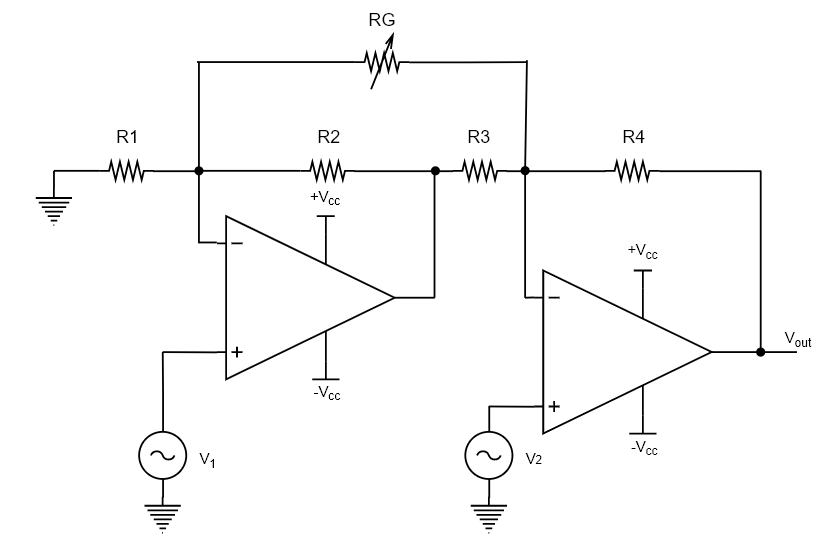
\includegraphics[width=0.9\textwidth]{../EJ4/resources/instrumental_2opamp_adjgain.png}
	\caption{Amplificador de instrumentaci\'on con ganancia ajustable}
   	\label{fig:EJ4_2opamp_adjgain}
\end{figure}

Del circuito anterior se deduce la ganancia, seg\'un la siguiente ecuaci\'on:

\begin{equation}
v_{out} = v_d \cdot \left( 1+\frac{R_2}{R_1}+\frac{2R_2}{R_G} \right)
\end{equation}

De esta forma, la ganancia tendr\'a una dependencia no lineal respecto de la resistencia variable $R_G$.

\section{Selecci\'on de componentes}




%\begin{figure}[H]
%    \centering
%    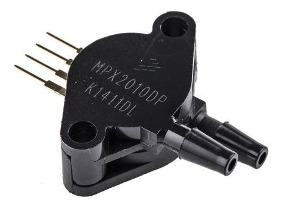
\includegraphics[width=0.9\textwidth]{../EJ4/resources/mpx2010dp.png}
%	\caption{Circuito l\'ogico}
%    \label{fig:ej4_circuito_logico}
%\end{figure}